\documentclass[]{article}
\usepackage{lmodern}
\usepackage{amssymb,amsmath}
\usepackage{ifxetex,ifluatex}
\usepackage{fixltx2e} % provides \textsubscript
\ifnum 0\ifxetex 1\fi\ifluatex 1\fi=0 % if pdftex
  \usepackage[T1]{fontenc}
  \usepackage[utf8]{inputenc}
\else % if luatex or xelatex
  \ifxetex
    \usepackage{mathspec}
  \else
    \usepackage{fontspec}
  \fi
  \defaultfontfeatures{Ligatures=TeX,Scale=MatchLowercase}
\fi
% use upquote if available, for straight quotes in verbatim environments
\IfFileExists{upquote.sty}{\usepackage{upquote}}{}
% use microtype if available
\IfFileExists{microtype.sty}{%
\usepackage{microtype}
\UseMicrotypeSet[protrusion]{basicmath} % disable protrusion for tt fonts
}{}
\usepackage[margin=1in]{geometry}
\usepackage{hyperref}
\hypersetup{unicode=true,
            pdftitle={Displacement effects and implications of Large-Scale Marine Protected Areas},
            pdfborder={0 0 0},
            breaklinks=true}
\urlstyle{same}  % don't use monospace font for urls
\usepackage{natbib}
\bibliographystyle{nature}
\usepackage{longtable,booktabs}
\usepackage{graphicx,grffile}
\makeatletter
\def\maxwidth{\ifdim\Gin@nat@width>\linewidth\linewidth\else\Gin@nat@width\fi}
\def\maxheight{\ifdim\Gin@nat@height>\textheight\textheight\else\Gin@nat@height\fi}
\makeatother
% Scale images if necessary, so that they will not overflow the page
% margins by default, and it is still possible to overwrite the defaults
% using explicit options in \includegraphics[width, height, ...]{}
\setkeys{Gin}{width=\maxwidth,height=\maxheight,keepaspectratio}
\IfFileExists{parskip.sty}{%
\usepackage{parskip}
}{% else
\setlength{\parindent}{0pt}
\setlength{\parskip}{6pt plus 2pt minus 1pt}
}
\setlength{\emergencystretch}{3em}  % prevent overfull lines
\providecommand{\tightlist}{%
  \setlength{\itemsep}{0pt}\setlength{\parskip}{0pt}}
\setcounter{secnumdepth}{0}
% Redefines (sub)paragraphs to behave more like sections
\ifx\paragraph\undefined\else
\let\oldparagraph\paragraph
\renewcommand{\paragraph}[1]{\oldparagraph{#1}\mbox{}}
\fi
\ifx\subparagraph\undefined\else
\let\oldsubparagraph\subparagraph
\renewcommand{\subparagraph}[1]{\oldsubparagraph{#1}\mbox{}}
\fi

%%% Use protect on footnotes to avoid problems with footnotes in titles
\let\rmarkdownfootnote\footnote%
\def\footnote{\protect\rmarkdownfootnote}

%%% Change title format to be more compact
\usepackage{titling}

% Create subtitle command for use in maketitle
\newcommand{\subtitle}[1]{
  \posttitle{
    \begin{center}\large#1\end{center}
    }
}

\setlength{\droptitle}{-2em}
  \title{Displacement effects and implications of Large-Scale Marine Protected
Areas}
  \pretitle{\vspace{\droptitle}\centering\huge}
  \posttitle{\par}
  \author{Juan Carlos Villaseñor-Derbez \textsuperscript{1} John Lynham
\textsuperscript{2}}
  \preauthor{\centering\large\emph}
  \postauthor{\par}
  \predate{\centering\large\emph}
  \postdate{\par}
  \date{\textsuperscript{1} Bren School of Environmental Science \& Management,
University of California, Santa Barbara \textsuperscript{2} Department
of Economics, Saunders Hall 532, University of Hawai`i at Manoa}

\usepackage{float}
\floatplacement{figure}{H}

\usepackage{amsthm}
\newtheorem{theorem}{Theorem}
\newtheorem{lemma}{Lemma}
\theoremstyle{definition}
\newtheorem{definition}{Definition}
\newtheorem{corollary}{Corollary}
\newtheorem{proposition}{Proposition}
\theoremstyle{definition}
\newtheorem{example}{Example}
\theoremstyle{definition}
\newtheorem{exercise}{Exercise}
\theoremstyle{remark}
\newtheorem*{remark}{Remark}
\newtheorem*{solution}{Solution}
\begin{document}
\maketitle
\begin{abstract}
Large-scale Marine Protected Areas (LSMPAs) have seen a significant
increase over the last years. Literature shows that fishing effort is
effectively eliminated in this protected areas upon implementation. The
benefits of reducing effort have been largely studied, and include
increases in abundance, biomass, and diversity within the bounded
regions. In terms of the fishing implication, no-take zones may produce
spillover that provide fish for outside areas. The implications of
displacement of fishing effort are not yet fully understood. Evidence
suggests that fishing effort re-distributes along the borders of the
MPA, following an ideal free distribution. Novel data products allow us
to track fishing effort at the vessel-level, allowing us to identify
changes in behavior at both the fleet and vessel level. This papers
evaluates the implications of implementing a LMPA, the Phoenix Islands
Protected Area (PIPA). We evaluate changes in fishing effort, and track
vessels to see where they go after the implementation of PIPA. Our
results show that vessels in the effected region increase fishing effort
after the implementation of PIPA. THey are redistributed to X. These
findings have major implications for MPA implementation, especially as
countries rush to meet the goals of 10\% ocean protection as mandated by
the SDG.
\end{abstract}

{
\setcounter{tocdepth}{4}
\tableofcontents
}
\emph{Last update: 2018-09-07}

\section{Introduction}\label{introduction}

The rest of the paper is outlined as follows: Section \ref{background}
provides further information about PIPA and Palau, section \ref{methods}
describes our data and empirical strategy, section \ref{results}
presents our results, in section \ref{discussion} we discuss our
findings and provide management recommendations.

\section{Background}\label{background}

\section{Methods}\label{methods}

\subsection{Data}\label{data}

The Global Fishing Watch (GFW) data contain 235 vessels that have fished
within PIPA waters \footnote{Perhaps some of these vessels only fished
  there for a couple hours one year. Therefore, I would need to further
  identify which ones were transient vs constant fishing events using
  some cutoff. For now, I run regressions for all vessels and for
  vessels that fly the Kiribati flag (n = 12). The true number of
  impacted vessels must lie between these two groups, but it provides a
  starting point.}. From these, 206 did so at least once before 2015.

\begin{table}

\caption{\label{tab:unnamed-chunk-3}Mean fishing hours for each gear before and after}
\centering
\begin{tabular}[t]{l|l|r|r|r}
\hline
Gear & Treated & Before & After & Change (A / B)\\
\hline
drifting\_longlines & FALSE & 484.47512 & 470.7382 & 0.9716458\\
\hline
drifting\_longlines & TRUE & 545.68460 & 523.5596 & 0.9594546\\
\hline
purse\_seines & FALSE & 59.64877 & 160.7945 & 2.6956886\\
\hline
purse\_seines & TRUE & 55.30178 & 149.9978 & 2.7123509\\
\hline
\end{tabular}
\end{table}

\begin{table}

\caption{\label{tab:unnamed-chunk-4}Number of fishing vessels (identified by mmsi) for each gear before and after PIPA implementation.}
\centering
\begin{tabular}[t]{l|l|r|r|r}
\hline
Gear & Treated & Before & After & Change (A / B)\\
\hline
drifting\_longlines & FALSE & 105 & 218 & 2.0761905\\
\hline
drifting\_longlines & TRUE & 139 & 118 & 0.8489209\\
\hline
purse\_seines & FALSE & 49 & 89 & 1.8163265\\
\hline
purse\_seines & TRUE & 78 & 81 & 1.0384615\\
\hline
\end{tabular}
\end{table}

Then, I look at the entire fishing effort of vessels that fished at
least once in PIPA before 2015. In other words, I use GFW data to track
vessel-level activities inside and outside PIPA before and after 2015.
However, all boats included in this case fished at least once in PIPA
before 2015 (\emph{i.e.} no control group). First I look at vessels
whose \texttt{mmsi} code starts with \texttt{529}, indicating that they
come from Kiribati \footnote{link:
  \url{http://www.vtexplorer.com/mmsi-mid-codes-en/}}. The overall
pattern for fishing time (total and mean) show a downward trend that
initiated well before 2015 (Fig. \ref{fig:kir_vessels}). The number of
vessels as given by unique mmsi numbers shows a maximum near the end of
2014, and then decreases after 2015.

\subsection{Analysis}\label{analysis}

\subsubsection{To do}\label{to-do}

\begin{itemize}
\tightlist
\item
  Divide pipa vessels by type of boat (longline vs.~purse seine)
\item
  Identify two counterfactuals:

  \begin{itemize}
  \tightlist
  \item
    A:

    \begin{itemize}
    \tightlist
    \item
      PNA
    \item
      similar vessel
    \item
      never fished inside PIPA -B:
    \item
      Taiwan
    \item
      Never in PNA
    \item
      Similar region?
    \end{itemize}
  \end{itemize}
\end{itemize}

Has effort increased?

\begin{itemize}
\tightlist
\item
  Change in fishing hours before vs after
\item
  Change in total hours before vs after
\item
  Change in distance before vs after
\item
  Where do PIPA vessels go?
\item
  How many were transient vs local?
\end{itemize}

Has search time increased?

\begin{itemize}
\tightlist
\item
  Distance between fishing points before vs.~after
\item
  Prop hour fishing before vs after
\item
  Time between fishing points before vs.~after
\end{itemize}

The current approach is to estimate what percentage of fishing effort
from the PNA was displaced by PIPA and use this to infer something about
Palau. While this provides a measure of the displacement, it does not
fully address the possibility of costs increasing. I believ we can use
individual tracks (as opposed to just the gridded effort) and obtain
show how their behavior changed (\emph{i.e.} are they fishing further
away, are they fishing more, where are they now?).

\subsubsection{Model specifications}\label{model-specifications}

Our model specification uses a difference-in-differences approach. In
this case, we interact the before-after dummy with a treatment dummy.
The treatment-control groups follow our definition in the data
description. The model takes the form of:

\[
H_{ijk} = \alpha + \beta Post_i \times Treat + \mu_j + \phi_k + \epsilon_{ijk}
\]

\section{Results}\label{results}

In this section I present some of the preliminary results of regressions
similar to what you have conducted for US MNMs using hours as an
estimate of fishing effort. First, I explore patterns of fishing effort
only inside PIPA (Fig. \ref{fig:blue_para}). Consistent with the blue
paradox \citep{mcdermott_2018}, we see an increase in the number of
vessels, total hours, mean hours, and number of data points between 2014
and 2015. Shortly after that, all measures decrease in 2015.

\begin{figure}
\centering
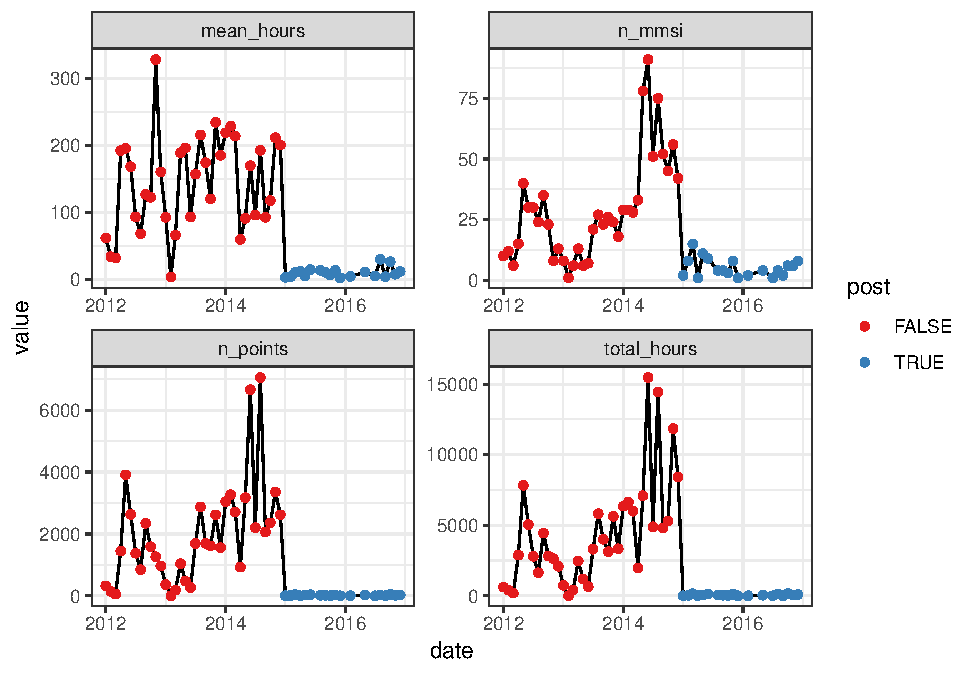
\includegraphics{C:/Users/JC/Documents/GitHub/MPA_displacement/docs/Manuscript_files/figure-latex/unnamed-chunk-5-1.pdf}
\caption{\label{fig:unnamed-chunk-5}\label{fig:blue_para}Monthly hours,
number of vessels, and data points observed inside PIPA. These clearly
show the blue-paradox effect.}
\end{figure}

\clearpage

Given the similar trends observed in total fishing hours and mean
fishing hours, I calculate total fishing hours at the year-month-vessel
level and regress that on a \texttt{post} dummy that indicates years
before or after 2015, which is interacted with a \texttt{treated} dummy
that indicates if vessels fished at least once within PIPA or only in
PNA waters. Results of this regression are presented in Table
\ref{tab:kir_vessels}. In this table, column (1) presents the regression
only against the policy dummy, column (2) includes month fixed effects,
column (3) includes month and year fixed effects, and column (4)
includes month, year, and vessel fixed effects. All three specifications
show negative coefficients. The full model explains 71\% of the variance
in monthly fishing hours by vessel. This specification has the lowest
policy coefficient (labeled \texttt{post}), and it is not different from
zero at the \(\alpha = 0.05\) level.

\begin{figure}
\centering
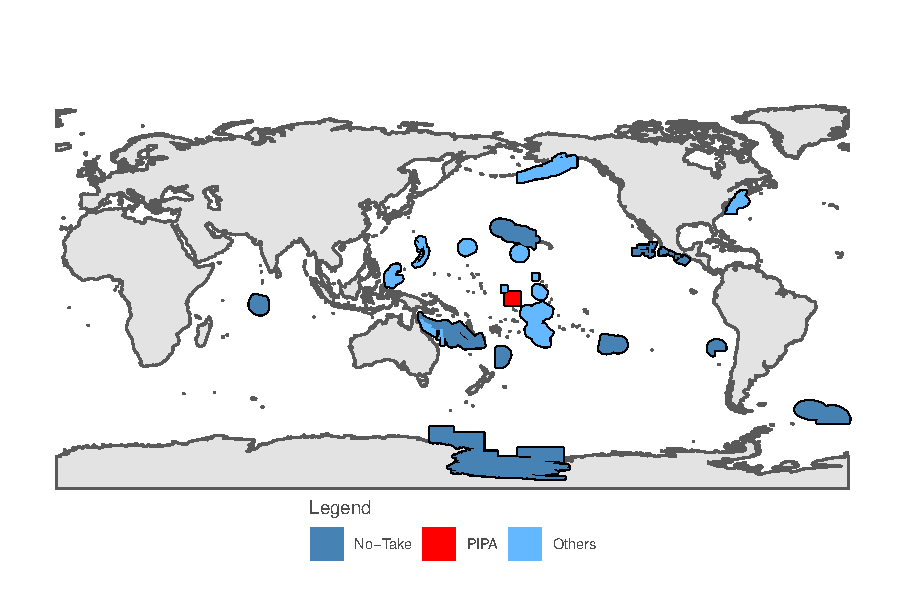
\includegraphics{C:/Users/JC/Documents/GitHub/MPA_displacement/docs/Manuscript_files/figure-latex/unnamed-chunk-6-1.pdf}
\caption{\label{fig:unnamed-chunk-6}\label{fig:kir_vessels}Fishing hours and
number of 12 Kiribati vessels from 2012 - 2016 that at some point fished
inside PIPA.}
\end{figure}

\begin{table}[!htbp] \centering 
  \caption{\label{tab:kir_vessels}Fishing hours from GFW for vessels flying Kiribati flag (n = 12). Asterisks indicate significance levels. Numbers in parenthesis represent heteroskedastic-robuste standard errors.} 
  \label{} 
\begin{tabular}{@{\extracolsep{5pt}}lcccc} 
\\[-1.8ex]\hline 
\hline \\[-1.8ex] 
 & \multicolumn{4}{c}{\textit{Dependent variable:}} \\ 
\cline{2-5} 
\\[-1.8ex] & \multicolumn{4}{c}{hours} \\ 
\\[-1.8ex] & (1) & (2) & (3) & (4)\\ 
\hline \\[-1.8ex] 
 post & 70.279$^{***}$ & 71.066$^{***}$ & 83.322$^{***}$ & 54.074$^{***}$ \\ 
  & (8.951) & (8.856) & (11.471) & (12.832) \\ 
  & & & & \\ 
 treated & $-$26.777 & $-$27.119 & $-$30.234$^{*}$ & $-$37.149 \\ 
  & (17.881) & (17.137) & (17.434) & (40.248) \\ 
  & & & & \\ 
 post:treated &  &  &  &  \\ 
  &  &  &  &  \\ 
  & & & & \\ 
 Constant & 81.770$^{***}$ & 88.095$^{***}$ & 70.812$^{***}$ & 126.560$^{***}$ \\ 
  & (18.737) & (23.142) & (24.053) & (34.921) \\ 
  & & & & \\ 
\hline \\[-1.8ex] 
Month FE & No & Yes & Yes & Yes \\ 
Year FE & No & No & Yes & Yes \\ 
Vessel FE & No & No & No & Yes \\ 
Observations & 344 & 344 & 344 & 344 \\ 
R$^{2}$ & 0.170 & 0.191 & 0.219 & 0.383 \\ 
\hline 
\hline \\[-1.8ex] 
\textit{Note:}  & \multicolumn{4}{r}{$^{*}$p$<$0.1; $^{**}$p$<$0.05; $^{***}$p$<$0.01} \\ 
\end{tabular} 
\end{table}

\clearpage

I then repeat a similar analysis but for all fishing vessels that fished
at least once inside PIPA before 2015. In this case this likely
represents an underestimate of the effect, as it could include vessels
who once fished inside PIPA, but are not even in the region any more.
The number of unique mmsi codes (Fig. \ref{fig:all_vessels}) follows a
similar pattern as in the previous case. However, mean hours and total
hours show stable trends before and after. As opposed to only Kiribati
vessels who seemed to reduce the number of fishing hours, a similar
analysis of all vessels shows positive coefficients that are not
statistically significant (\(alpha < 0.05\)). Results of the regressions
are shown in Table \ref{tab:all_vessels}. Like before, column (1)
presents the regression only against the policy dummy, column (2)
includes month fixed effects, column (3) includes month and year fixed
effects, and column (4) includes month, year, and vessel fixed effects.

\begin{figure}
\centering
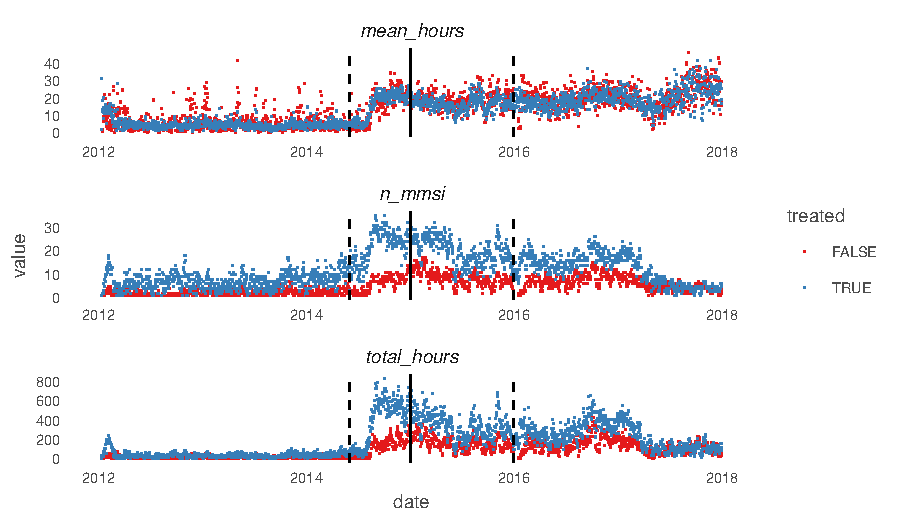
\includegraphics{C:/Users/JC/Documents/GitHub/MPA_displacement/docs/Manuscript_files/figure-latex/unnamed-chunk-8-1.pdf}
\caption{\label{fig:unnamed-chunk-8}\label{fig:all_vessels}Fishing hours and
number of vessels by month for all vessels that fished inside PIPA at
least once.}
\end{figure}

\begin{table}[!htbp] \centering 
  \caption{\label{tab:all_vessels}Fishing hours from GFW for all vessels (n = 206) that at some point fished in PIPA. Asterisks indicate significance levels. Numbers in parenthesis represent heteroskedastic-robuste standard errors.} 
  \label{} 
\begin{tabular}{@{\extracolsep{5pt}}lcccc} 
\\[-1.8ex]\hline 
\hline \\[-1.8ex] 
 & \multicolumn{4}{c}{\textit{Dependent variable:}} \\ 
\cline{2-5} 
\\[-1.8ex] & \multicolumn{4}{c}{hours} \\ 
\\[-1.8ex] & (1) & (2) & (3) & (4)\\ 
\hline \\[-1.8ex] 
 post & 45.766$^{***}$ & 45.268$^{***}$ & 41.959$^{***}$ & 45.596 \\ 
  & (6.534) & (6.504) & (8.779) &  \\ 
  & & & & \\ 
 treated & 50.000$^{***}$ & 51.321$^{***}$ & 50.749$^{***}$ & $-$457.705 \\ 
  & (6.771) & (6.759) & (6.813) &  \\ 
  & & & & \\ 
 postTRUE:treated & $-$59.473$^{***}$ & $-$58.530$^{***}$ & $-$57.494$^{***}$ & $-$21.059 \\ 
  & (8.463) & (8.432) & (8.491) &  \\ 
  & & & & \\ 
 Constant & 349.582$^{***}$ & 328.470$^{***}$ & 333.794$^{***}$ & 483.665 \\ 
  & (5.635) & (8.833) & (10.226) &  \\ 
  & & & & \\ 
\hline \\[-1.8ex] 
Month FE & No & Yes & Yes & Yes \\ 
Year FE & No & No & Yes & Yes \\ 
Vessel FE & No & No & No & Yes \\ 
Observations & 15,885 & 15,885 & 15,885 & 15,885 \\ 
R$^{2}$ & 0.004 & 0.011 & 0.011 & 0.632 \\ 
\hline 
\hline \\[-1.8ex] 
\textit{Note:}  & \multicolumn{4}{r}{$^{*}$p$<$0.1; $^{**}$p$<$0.05; $^{***}$p$<$0.01} \\ 
\end{tabular} 
\end{table}

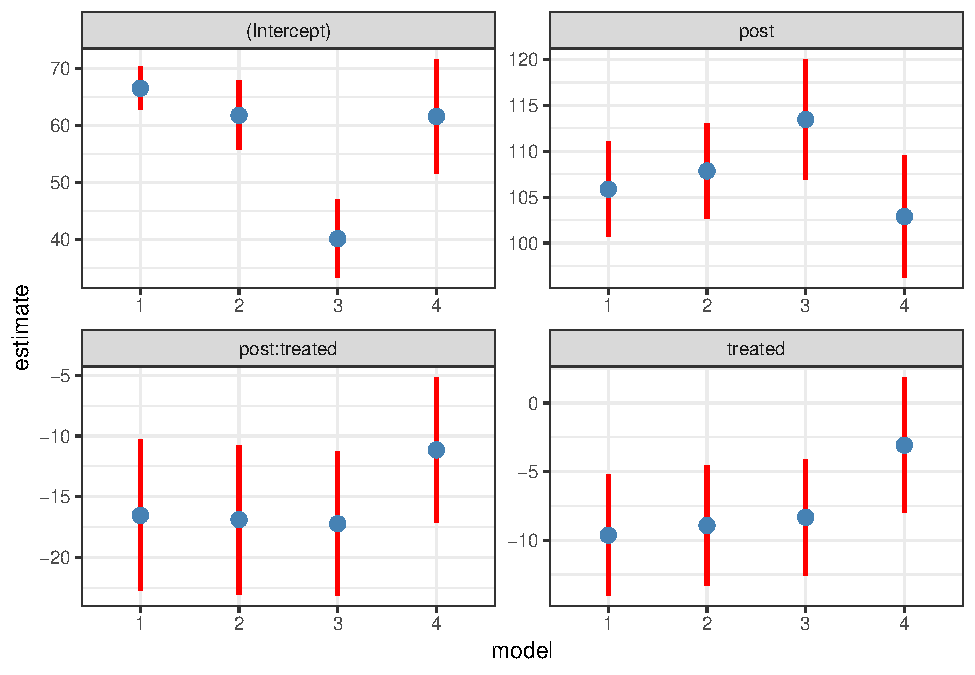
\includegraphics{C:/Users/JC/Documents/GitHub/MPA_displacement/docs/Manuscript_files/figure-latex/unnamed-chunk-10-1.pdf}

\section{Discusion}\label{discusion}

\clearpage

\subsubsection{Further work}\label{further-work}

\renewcommand\refname{References}
\bibliography{references.bib}


\end{document}
